% !TEX root = thesis_draft.tex

\section{Varying time-frequency analysis methods}

\subsection{Introduction}

Inter-brain synchrony (IBS) values are calculated on a frequency domain
representation of the original signals. Obtaining this frequency domain
representation requires making some methodological choices: you need to choose
a window of interest, a calculation method and a resolution. We assess how these
choices affect the final IBS values.

Ideally, the IBS values should be robust to slight changes in these parameters.
For the window of interest case, IBS values could presumably vary a bit as
the window could include or exclude cognitive processes that take a while to
start after the stimulus. But the other parameters are just technical details of
the time-frequency analysis process and should not have a big effect on the IBS
values when reasonably chosen.

\subsection{Methods}

To assess the effect of different windows of interest on the
results, we repeat the main frequency analysis using a window of half a second
before to one second after stimulus presentation, making full use of each
available pre-processed data point. To determine the effect of different
frequency analysis methods on the final results, we also repeat the (alpha band)
analysis using multitapers instead of a Hann taper. To find whether there is an
effect of resolution, we perform the frequency analysis both more often (for
each original data point, i.e. 512 times per second or approximately every 2 ms)
and less often (once every 20 ms). None of these variations are extreme, and all
could have been reasonably chosen for the main experiment instead.

For each of these variations, we first compare the averaged IBS values by
plotting the data and assess the significance using a linear mixed effect model.
If those do not show a difference at first glance, we further assess possible
differences in the underlying data structure by calculating correlations between
the values for different conditions and (where necessary) by plotting the data.
Correlations are calculated for each session, Fisher transformed
\parencite{fisher_frequency_1915}, averaged and transformed back.

\subsection{Results}

\subsubsection{Frequency analysis window size}

\begin{figure}[!htpb]
  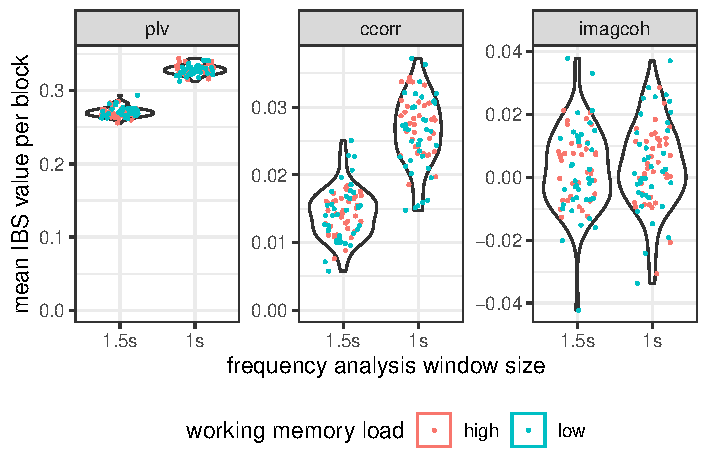
\includegraphics[width=\linewidth]{../stats/results/winsize.pdf}
  \caption{(Mean) alpha band inter-brain synchrony values are sensitive to different time windows of interest within a trial. The 1s window starts at the presentation of the stimuli, while the 1.5s window starts half a second earlier during fixation. Working memory load has no effect. Finally, the (mean) circular correlation and imaginary part of coherency values are both very close to zero considering they are on a scale from -1 to 1. The phase locking value is on a 0-1 scale.}
  \label{fig:winsize}
\end{figure}

We tested the effect of window size on IBS values by calculating the IBS
measures on overlapping windows of 1s and 1.5s respectively. Contrary to our
initial expectations, we found IBS values to be sensitive to changes
in frequency analysis window size. See Figure~\ref{fig:winsize}. The phase
locking value (PLV) significantly decreased when the larger window was used
($\chi^2$(1) = 29984, p < 0.001, $\Delta$AIC = 29982, $\Delta$BIC = 29971) and
so did the circular correlation (CCorr; $\chi^2$(1) = 1071, p < 0.001, $\Delta$AIC = 1069,
$\Delta$BIC = 1058), but no significant effect was found for the imaginary part
of coherency values (ImagCoh; $\chi^2$(1) = 2.27, n.s., $\Delta$AIC = 0.27,
$\Delta$BIC = 10.66).

\subsubsection{Frequency analysis taper}

\begin{figure}[!htpb]
  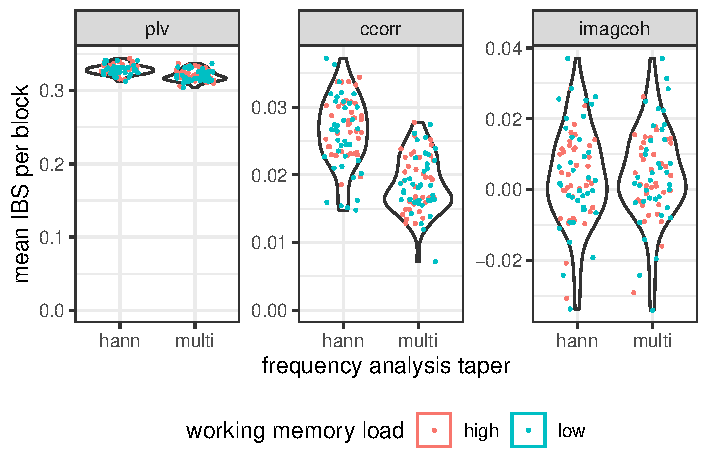
\includegraphics[width=\linewidth]{../stats/results/freqmethod.pdf}s
  \caption{Choice of taper matters when calculating (mean) `phase locking value', `circular correlation' and `imaginary part of coherency' inter-brain synchrony values for the alpha band. Working memory load has no influence.}
  \label{fig:freqmethod}
\end{figure}

\begin{figure}[!htpb]
  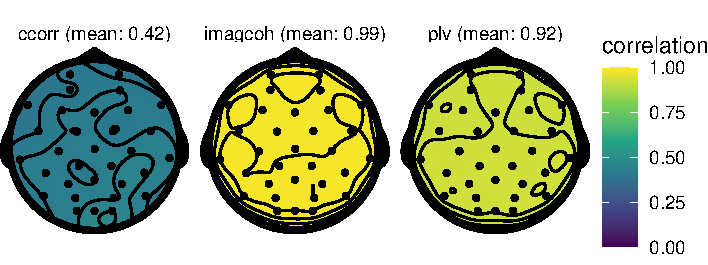
\includegraphics[width=\linewidth]{../stats/results/freqmethodcorr.pdf}
  \caption{When calculating phase locking value and circular correlation measures, the choice of taper alone can lead to inter-brain synchrony values different enough that they do not perfectly correlate with each other. Imaginary part of coherency values are less affected than circular correlations and phase locking values.}
  \label{fig:freqmethodcorr}
\end{figure}

To see the effect of taper choice on the frequency analysis, we compared the
IBS values obtained from spectra generated using a Hann taper and a multitaper.
As you can see in Figure~\ref{fig:freqmethod}, there is an effect of taper
choice on PLV synchrony values ($\chi^2$(1) = 626, p < 0.001, $\Delta$AIC = 624,
$\Delta$BIC = 614) and CCorr synchony values. ($\chi^2$(1) = 452, p < 0.001,
$\Delta$AIC = 450, $\Delta$BIC = 440). In both cases, the IBS value decreases a
bit when multitapers are used. Again, there is no significant effect on
ImagCoh synchrony values ($\chi^2$(1) = 0.51, n.s., $\Delta$AIC = 1.49,
$\Delta$BIC = 12.4). When we compare how values calculated using the different
methods correlate (Figure \ref{fig:freqmethodcorr}), we again see that IBS value
calculation is sensitive to choice of taper contrary to our hypothesis. The
CCorr measure is especially affected with a mean correlation of 0.42 across
sessions and electrodes.

\subsubsection{Frequency analysis resolution}

\begin{figure}[!htpb]
  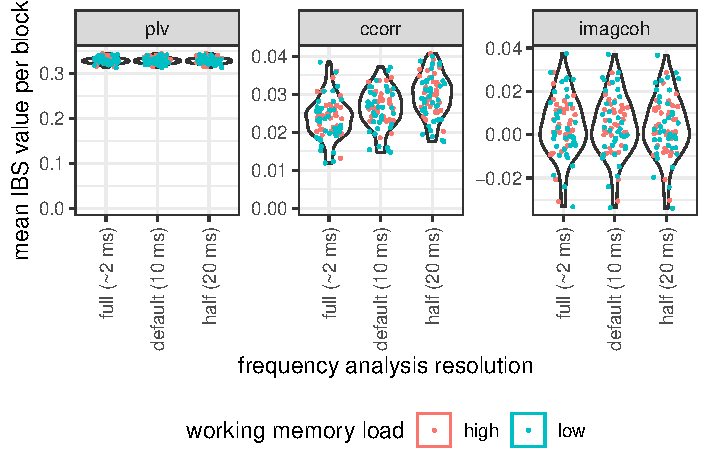
\includegraphics[width=\linewidth]{../stats/results/resolution.pdf}
  \caption{Mean inter-brain synchrony values do not appear to vary much with resolution, with the exception of a slight effect on circular correlation values.}
  \label{fig:resolution}
\end{figure}

\begin{figure}[!htpb]
  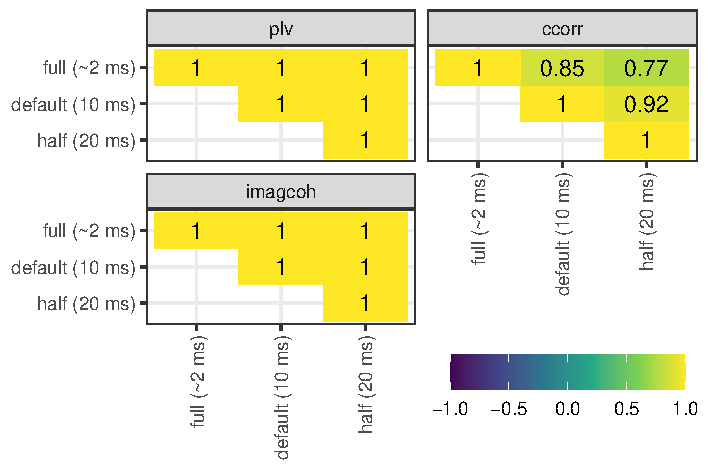
\includegraphics[width=\linewidth]{../stats/results/resolutioncorr.pdf}
  \caption{The phase locking value and imaginary part of coherency measures are robust to being calculated on frequency spectra of different resolutions. Circular correlation values, in contrast, will not correlate perfectly when comparing values across resolutions. Figure~\ref{fig:resolutionapp} shows the full underlying data for the CCorr case where $r$ = 0.77.}
  \label{fig:resolutioncorr}
\end{figure}

We now turn to a less discussed parameter of the frequency analysis: the
resolution of the resulting spectrum. At first sight, there does not appear to
be an effect of resolution on IBS values (Figure~\ref{fig:resolution}). When
using the resolution as a continuous parameter ($\frac{1000}{512}$ ms, 10 ms or
20 ms), statistics confirm this for the PLV ($\chi^2$(1) = 0.145, n.s.,
$\Delta$AIC = 1.85, $\Delta$BIC = 13.2) and ImagCoh ($\chi^2$(1) = 0, n.s.,
$\Delta$AIC = 2.0, $\Delta$BIC = 13.3) measures, but report a significant
positive (though small) effect of resolution on CCorr synchrony values
($\chi^2$(1) = 7.4, p < 0.01, $\Delta$AIC = 5.4, $\Delta$BIC = -5.9).

Looking into it further, we see that CCorr values in fact
correlate much worse across resolutions than the other measures
(see Figure~\ref{fig:resolutioncorr}). This is unexpected when varying such a
`boring' parameter as resolution, which you normally do not think twice about
when choosing it.


\subsection{Discussion}

An effect of window size was found for the CCorr and PLV measures, but not for
the ImagCoh measure. In hindsight, the effect of window size is not that
surprising, as all measure definitions weigh each data point equally and one
third of the data is new for the 1.5s window of interest. Still, as all IBS
present in the short window is also present in the longer window, we would not
expect any effects to change direction, especially as the extra half second is
time in which the participants are `only' watching the fixation point. This
indeed seems to be the case.

The lack of an effect on the ImagCoh measure could mean that the underlying
functional (dis)similarities that the other measures now pick up on are in phase
in both signals. But it could also just indicate a lack of sensitivity of the
ImagCoh measure.

Using multitapers also changed CCorr and PLV values. This could
be because multitapers are ill suited to performing a frequency analysis of
low-frequency data \parencite[p.~203]{cohen_analyzing_2014}. (Which the alpha
band (9--14 Hz) data used for this experiment is.) But that does not explain why
the CCorr and PLV measures are again more affected than the ImagCoh measure.
Especially the CCorr value with a mean correlation when comparing tapers of only
0.42 across sessions and electrodes (Figure~\ref{fig:freqmethodcorr}).

As expected, no effect of resolution was found for the PLV and ImagCoh measures.
In contrast, the CCorr values are not stable when calculated for different
resolutions. While you could still argue that the variance was reasonable for
the multitaper case, it seems conceptually bad for a change in sampling rate to
have a big effect on an IBS value when the underlying data has not
changed. So it is worth discussing the big variance introduced by the CCorr
measure in more detail.

\subsubsection{Stability of circular correlation synchrony values}

We found the CCorr values to change quite a bit when only small
changes to the frequency analysis process where made. Apparently, contrary to
PLV and ImagCoh, the values do not converge to a single stable value. This is
surpising, because \textcite{burgess_interpretation_2013} previously found CCorr
to be more robust than other measures. \textcite{pauen_circular_2013} also found
it to at least not perform worse than PLV.

\begin{algorithm}[!htpb]
  \caption{Calculates a robust circular correlation coefficient. Based on \textcite{mahmood_robust_2022}'s work, using the (univariate) dispersion measure from \textcite[p.~28]{pewsey_circular_2013}.}
  \begin{algorithmic}
  \Require $\phi, \psi$ \Comment The input signals (phases).
  \State $n \gets \text{length of }\phi$
  \State $n' \gets n \cdot 0.95$ \Comment How many data points to keep?
  \While{$n > n'$}
    \For{$i \in 1 \ldots n$}
      \State $d_i \gets \sum\limits_{j = 0}^n \text{dist}(\phi_i, \phi_j) + \text{dist}(\psi_i, \psi_j)$
    \EndFor
    \State $i \gets \text{argmax}(d)$ \Comment The point that maximizes the distances.
    \State remove $\phi_i$ and $\psi_i$ from $\phi$ and $\psi$ respectively
    \State $n \gets n - 1$
   \EndWhile
   \State\Return $\text{CCorr}(\phi, \psi)$ \Comment As defined in Equation~\ref{eq:ccorr}.
  \end{algorithmic}
  \label{alg:robust}
\end{algorithm}

When investigating why the CCorr varies this much, we
hypothesised it could be overly influenced by outliers.
\textcite{mahmood_robust_2022} proposes a robust version of the CCorr measure
which removes values that ``lie far away from the majority of the circular data
based on the circular geometry theory''.
\citeauthor{mahmood_robust_2022} shows using simulations that his `trimmed
robust circular correlation' measure succesfully reduces the influence of
outliers. That makes it ideal to test our hypothesis. But sadly, not enough
information is provided to unambiguously reproduce
\citeauthor{mahmood_robust_2022}'s method. While `lying far away' is
well-defined for univariate circular data using the dispersion measure
\parencite[p.~26]{pewsey_circular_2013}, robust correlations need to have a way
of detecting bivariate outliers \parencite[p.~12]{maronna_robust_2019} as points
can be outliers while not being extreme in any dimension by itself. To the best
of my knowledge, such methods have only been published for normal correlations
\parencite[chapter~6]{bebbington_method_1978,shevlyakov_robust_2010,maronna_robust_2019}, not circular ones.
As a result, it is likely that \citeauthor{mahmood_robust_2022} instead only
considered outliers that are isolated in a single dimension. Working with this
assumption, we defined the robust circular correlation as given in
Algorithm~\ref{alg:robust}.

The resulting algorithm is slow, so it was only applied to the data sets
obtained using the standard frequency analysis resolution (10 ms) and half the
resolution (20 ms). It results in circular correlation values higher (around
0.11) than those found previously (around 0.03; Figure~\ref{fig:resolution}).
When correlating the IBS values for the different resolutions, we get a (mean)
correlation of 0.87, which is close to the value of 0.92 we got for normal
CCorr (Figure~\ref{fig:resolutioncorr}). But as it is still not
`1', our robust circular correlation measure clearly did nothing to resolve the
circular correlation stability issue. Apparently, outliers are not the problem.

\begin{figure}[!htpb]
  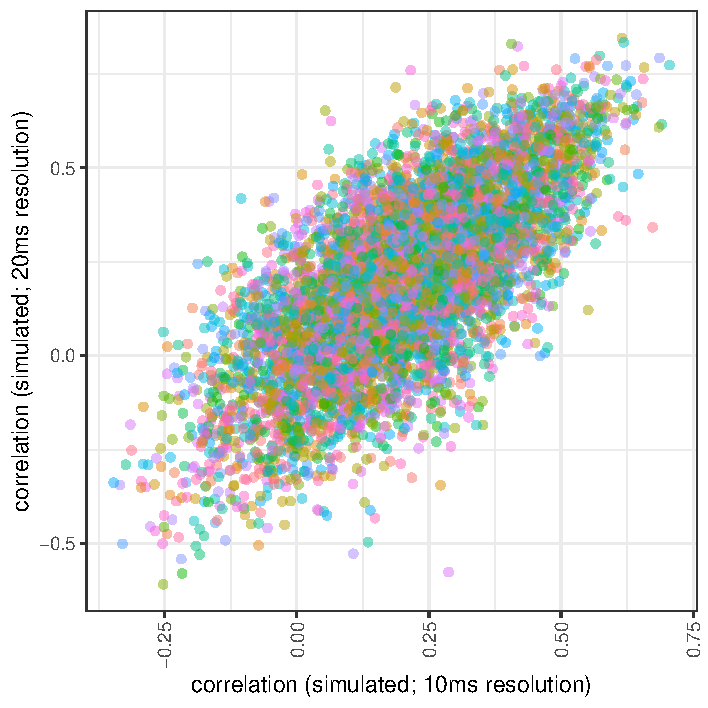
\includegraphics[width=\linewidth]{../stats/results/corsimulation.pdf}
  \caption{The correlation of simulated (correlated) normal data before and after downsampling. Simulates a single session with 32 electrodes (each represented by a different color) for 180 trials. The result matches the emperical data in Figure~\ref{fig:resolutionapp} quite well. This illustrates that the circular correlation stability issue also exists for normal correlations.}
  \label{fig:corsimulation}
\end{figure}

As sampling at half the resolution is equivalent to just leaving out every
second data point, the issue is also unlikely to be caused by more sophisticated
frequency analysis issues like spectral leakage. Instead, after further
investigation, the problem seems to be inherent to correlation measures. This is
most easily demonstrated with a simulation. We replace the CCorr measure with a
Pearson correlation, and the underlying phase signals by data drawn from a
multi-variate normal distribution while making sure the signals are somewhat
correlated. We also calculate correlations after downsampling our `signals' by
half. The result can be seen in Figure~\ref{fig:corsimulation}. Clearly, the
correlation ($r=0.72$) between CCorrs of different resolutions is not perfect
when using normal correlations to simulate them either.

On the one hand, this is good news. Normal correlations are not fundamentally
flawed, so there is no reason not to use the CCorr measure either. On the other
hand, it cannot be denied that CCorr values are less stable than PLV or ImagCoh
values. As such, more care is required when interpreting raw values, as we will
do in the time course analysis section. Permutation tests are an elegant
solution to the problem: as they encounter the variation issue also during null
distribution construction, it is automatically taken into account when
determining the final p-value.
